% Overview of FCT (Section IV). Needs \usepackage{tikz} and
% \usetikzlibrary{arrows.meta,positioning,calc,fit,backgrounds}.
% Thumbnails: figures/ov/*.png (a Kvasir-SEG training image, its two flips and its label).
\definecolor{flipc}{HTML}{2A78D6}
\definecolor{upc}{HTML}{EB6834}
\begin{tikzpicture}[
  font=\footnotesize, >={Stealth[length=4.2pt,width=3.8pt]},
  img/.style={inner sep=0pt, draw=black!35, line width=0.3pt},
  net/.style={draw=black!70, line width=0.5pt, fill=black!4, rounded corners=1.5pt,
              minimum width=9mm, minimum height=7mm, align=center},
  map/.style={draw=black!70, line width=0.5pt, fill=white, minimum width=8mm, minimum height=7mm},
  sup/.style={draw=black!60, line width=0.4pt, fill=black!4, rounded corners=1.5pt,
              minimum height=5.5mm, inner xsep=2.5pt, align=center},
  flow/.style={->, line width=0.5pt, black!75},
  pull/.style={->, line width=1.2pt},
  lab/.style={font=\scriptsize, black!85, align=center},
]
  \def\th{10.5mm}
  % ---- inputs: the image and its two flips -------------------------------------
  \node[img] (xh) at (0, 1.45)  {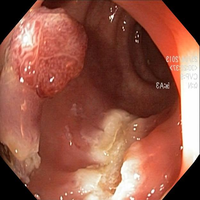
\includegraphics[width=\th]{figures/ov/xh.png}};
  \node[img] (x)  at (0, 0)     {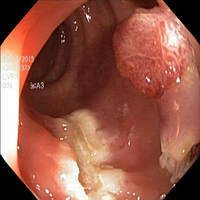
\includegraphics[width=\th]{figures/ov/x.png}};
  \node[img] (xv) at (0, -1.45) {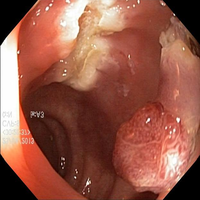
\includegraphics[width=\th]{figures/ov/xv.png}};
  \node[lab, left=1.2mm of xh] {$T_h x$};
  \node[lab, left=1.2mm of x]  {$x$};
  \node[lab, left=1.2mm of xv] {$T_v x$};
  % ---- one network, three passes ------------------------------------------------
  \node[net] (fh) at (1.6, 1.45)  {$f$};
  \node[net] (fo) at (1.6, 0)     {$f$};
  \node[net] (fv) at (1.6, -1.45) {$f$};
  \draw[flow] (xh) -- (fh); \draw[flow] (x) -- (fo); \draw[flow] (xv) -- (fv);
  \begin{scope}[on background layer]
    \node[draw=black!35, dashed, line width=0.4pt, rounded corners=2pt, fit=(fh)(fv), inner sep=2.2mm] (shared) {};
  \end{scope}
  \node[lab, below=0.6mm of shared] {shared weights,\\ same depth mask};
  % ---- logits in the upright frame -----------------------------------------------
  \node[map] (zh) at (3.45, 1.45)  {$z^{h}$};
  \node[map] (zo) at (3.45, 0)     {$z^{o}$};
  \node[map] (zv) at (3.45, -1.45) {$z^{v}$};
  \draw[flow] (fh) -- node[lab, above, pos=0.62] {$T_h^{-1}$} (zh);
  \draw[flow] (fo) -- (zo);
  \draw[flow] (fv) -- node[lab, above, pos=0.62] {$T_v^{-1}$} (zv);
  % ---- (1) the three supervised views ---------------------------------------------
  \node[sup] (sh) at (5.2, 1.45)  {$\tfrac13\mathcal{L}_{\mathrm{host}}$};
  \node[sup] (so) at (5.2, 0)     {$\tfrac13\mathcal{L}_{\mathrm{host}}$};
  \node[sup] (sv) at (5.2, -1.45) {$\tfrac13\mathcal{L}_{\mathrm{host}}$};
  \draw[flow] (zh) -- (sh); \draw[flow] (zo) -- (so); \draw[flow] (zv) -- (sv);
  \node[img] (y) at (6.85, 0) {
\includegraphics[width=\th]{figures/ov/y.png}};
  \node[lab, below=0.6mm of y] {label $y$};
  \draw[flow, black!45] (y.north west) -- (sh.east);
  \draw[flow, black!45] (y.west) -- (so.east);
  \draw[flow, black!45] (y.south west) -- (sv.east);
  \node[lab, above=1.4mm of sh, xshift=4mm] {(1) three supervised views};
  % ---- (2) the consistency term between the views' probabilities -----------------
  \node[map] (po) at (8.75, 0)     {$p^{o}$};
  \node[map] (ph) at (10.95, 1.15) {$p^{h}$};
  \node[map] (pv) at (10.95, -1.15) {$p^{v}$};
  \draw[pull, flipc] (po.north) to[bend left=28] node[lab, above left, pos=0.45, xshift=1mm] {$C_h$, weight $w_h$} (ph.west);
  \draw[pull, upc]   (ph.south) to[bend left=28] (po.east);
  \draw[pull, flipc] (po.south) to[bend right=28] node[lab, below left, pos=0.45, xshift=1mm] {$C_v$, weight $w_v$} (pv.west);
  \draw[pull, upc]   (pv.north) to[bend right=28] (po.east);
  \node[lab] at (9.95, 0.47) {$U$, gate $g$};
  \node[lab] at (9.85, 2.25) {(2) label-aware consistency, $p=\sigma(z)$};
  \node[lab, anchor=west] at (11.55, 0.35) {\textcolor{flipc}{\rule[0.5ex]{3mm}{1.2pt}} flipped views:};
  \node[lab, anchor=west] at (11.55, 0.0) {lag or margin};
  \node[lab, anchor=west] at (11.55, -0.45) {\textcolor{upc}{\rule[0.5ex]{3mm}{1.2pt}} upright view:};
  \node[lab, anchor=west] at (11.55, -0.8) {best flip, gated};
  \node[lab] at (9.85, -2.2) {arrow: detached target $\to$ view it moves};
\end{tikzpicture}
